\documentclass[]{article}
\usepackage{lmodern}
\usepackage{amssymb,amsmath}
\usepackage{ifxetex,ifluatex}
\usepackage{fixltx2e} % provides \textsubscript
\ifnum 0\ifxetex 1\fi\ifluatex 1\fi=0 % if pdftex
  \usepackage[T1]{fontenc}
  \usepackage[utf8]{inputenc}
\else % if luatex or xelatex
  \ifxetex
    \usepackage{mathspec}
  \else
    \usepackage{fontspec}
  \fi
  \defaultfontfeatures{Ligatures=TeX,Scale=MatchLowercase}
\fi
% use upquote if available, for straight quotes in verbatim environments
\IfFileExists{upquote.sty}{\usepackage{upquote}}{}
% use microtype if available
\IfFileExists{microtype.sty}{%
\usepackage{microtype}
\UseMicrotypeSet[protrusion]{basicmath} % disable protrusion for tt fonts
}{}
\usepackage[margin=1in]{geometry}
\usepackage{hyperref}
\hypersetup{unicode=true,
            pdftitle={Homework 12},
            pdfauthor={Christophe Hunt},
            pdfborder={0 0 0},
            breaklinks=true}
\urlstyle{same}  % don't use monospace font for urls
\usepackage{color}
\usepackage{fancyvrb}
\newcommand{\VerbBar}{|}
\newcommand{\VERB}{\Verb[commandchars=\\\{\}]}
\DefineVerbatimEnvironment{Highlighting}{Verbatim}{commandchars=\\\{\}}
% Add ',fontsize=\small' for more characters per line
\usepackage{framed}
\definecolor{shadecolor}{RGB}{248,248,248}
\newenvironment{Shaded}{\begin{snugshade}}{\end{snugshade}}
\newcommand{\KeywordTok}[1]{\textcolor[rgb]{0.13,0.29,0.53}{\textbf{{#1}}}}
\newcommand{\DataTypeTok}[1]{\textcolor[rgb]{0.13,0.29,0.53}{{#1}}}
\newcommand{\DecValTok}[1]{\textcolor[rgb]{0.00,0.00,0.81}{{#1}}}
\newcommand{\BaseNTok}[1]{\textcolor[rgb]{0.00,0.00,0.81}{{#1}}}
\newcommand{\FloatTok}[1]{\textcolor[rgb]{0.00,0.00,0.81}{{#1}}}
\newcommand{\ConstantTok}[1]{\textcolor[rgb]{0.00,0.00,0.00}{{#1}}}
\newcommand{\CharTok}[1]{\textcolor[rgb]{0.31,0.60,0.02}{{#1}}}
\newcommand{\SpecialCharTok}[1]{\textcolor[rgb]{0.00,0.00,0.00}{{#1}}}
\newcommand{\StringTok}[1]{\textcolor[rgb]{0.31,0.60,0.02}{{#1}}}
\newcommand{\VerbatimStringTok}[1]{\textcolor[rgb]{0.31,0.60,0.02}{{#1}}}
\newcommand{\SpecialStringTok}[1]{\textcolor[rgb]{0.31,0.60,0.02}{{#1}}}
\newcommand{\ImportTok}[1]{{#1}}
\newcommand{\CommentTok}[1]{\textcolor[rgb]{0.56,0.35,0.01}{\textit{{#1}}}}
\newcommand{\DocumentationTok}[1]{\textcolor[rgb]{0.56,0.35,0.01}{\textbf{\textit{{#1}}}}}
\newcommand{\AnnotationTok}[1]{\textcolor[rgb]{0.56,0.35,0.01}{\textbf{\textit{{#1}}}}}
\newcommand{\CommentVarTok}[1]{\textcolor[rgb]{0.56,0.35,0.01}{\textbf{\textit{{#1}}}}}
\newcommand{\OtherTok}[1]{\textcolor[rgb]{0.56,0.35,0.01}{{#1}}}
\newcommand{\FunctionTok}[1]{\textcolor[rgb]{0.00,0.00,0.00}{{#1}}}
\newcommand{\VariableTok}[1]{\textcolor[rgb]{0.00,0.00,0.00}{{#1}}}
\newcommand{\ControlFlowTok}[1]{\textcolor[rgb]{0.13,0.29,0.53}{\textbf{{#1}}}}
\newcommand{\OperatorTok}[1]{\textcolor[rgb]{0.81,0.36,0.00}{\textbf{{#1}}}}
\newcommand{\BuiltInTok}[1]{{#1}}
\newcommand{\ExtensionTok}[1]{{#1}}
\newcommand{\PreprocessorTok}[1]{\textcolor[rgb]{0.56,0.35,0.01}{\textit{{#1}}}}
\newcommand{\AttributeTok}[1]{\textcolor[rgb]{0.77,0.63,0.00}{{#1}}}
\newcommand{\RegionMarkerTok}[1]{{#1}}
\newcommand{\InformationTok}[1]{\textcolor[rgb]{0.56,0.35,0.01}{\textbf{\textit{{#1}}}}}
\newcommand{\WarningTok}[1]{\textcolor[rgb]{0.56,0.35,0.01}{\textbf{\textit{{#1}}}}}
\newcommand{\AlertTok}[1]{\textcolor[rgb]{0.94,0.16,0.16}{{#1}}}
\newcommand{\ErrorTok}[1]{\textcolor[rgb]{0.64,0.00,0.00}{\textbf{{#1}}}}
\newcommand{\NormalTok}[1]{{#1}}
\usepackage{graphicx,grffile}
\makeatletter
\def\maxwidth{\ifdim\Gin@nat@width>\linewidth\linewidth\else\Gin@nat@width\fi}
\def\maxheight{\ifdim\Gin@nat@height>\textheight\textheight\else\Gin@nat@height\fi}
\makeatother
% Scale images if necessary, so that they will not overflow the page
% margins by default, and it is still possible to overwrite the defaults
% using explicit options in \includegraphics[width, height, ...]{}
\setkeys{Gin}{width=\maxwidth,height=\maxheight,keepaspectratio}
\IfFileExists{parskip.sty}{%
\usepackage{parskip}
}{% else
\setlength{\parindent}{0pt}
\setlength{\parskip}{6pt plus 2pt minus 1pt}
}
\setlength{\emergencystretch}{3em}  % prevent overfull lines
\providecommand{\tightlist}{%
  \setlength{\itemsep}{0pt}\setlength{\parskip}{0pt}}
\setcounter{secnumdepth}{5}
% Redefines (sub)paragraphs to behave more like sections
\ifx\paragraph\undefined\else
\let\oldparagraph\paragraph
\renewcommand{\paragraph}[1]{\oldparagraph{#1}\mbox{}}
\fi
\ifx\subparagraph\undefined\else
\let\oldsubparagraph\subparagraph
\renewcommand{\subparagraph}[1]{\oldsubparagraph{#1}\mbox{}}
\fi

%%% Use protect on footnotes to avoid problems with footnotes in titles
\let\rmarkdownfootnote\footnote%
\def\footnote{\protect\rmarkdownfootnote}

%%% Change title format to be more compact
\usepackage{titling}

% Create subtitle command for use in maketitle
\newcommand{\subtitle}[1]{
  \posttitle{
    \begin{center}\large#1\end{center}
    }
}

\setlength{\droptitle}{-2em}
  \title{Homework 12}
  \pretitle{\vspace{\droptitle}\centering\huge}
  \posttitle{\par}
  \author{Christophe Hunt}
  \preauthor{\centering\large\emph}
  \postauthor{\par}
  \predate{\centering\large\emph}
  \postdate{\par}
  \date{April 27, 2017}

\usepackage{relsize}
\usepackage{setspace}
\usepackage{amsmath,amsfonts,amsthm}
\usepackage[sfdefault]{roboto}
\usepackage[T1]{fontenc}
\usepackage{float}
\usepackage{multirow}
\usepackage{mathtools}
\usepackage{tikz}

\begin{document}
\maketitle

{
\setcounter{tocdepth}{2}
\tableofcontents
}
\section{Assignment Introduction}\label{assignment-introduction}

Using the \(stats\) and \(boot\) libraries in R perform a
cross-validation experiment to observe the bias variance tradeoff.
You'll use the auto data set from previous assignments. This dataset has
392 observations across 5 variables. We want to fit a polynomial model
of various degrees using the \(glm\) function in R and then measure the
cross validation error using cv.glm function.

Fit various polynomial models to compute \(mpg\) as a function of the
other four variables
\(acceleration, weight, horsepower, and displacement\) using \(glm\)
function. For example:

\textbf{glm.fit=glm(mpg\textasciitilde{}poly(disp+hp+wt+acc,2),
data=auto)}\\
\textbf{cv.err5{[}2{]}=cv.glm(auto,glm.fit,K=5)\$delta{[}1{]}}

will fit a 2nd degree polynomial function between \(mpg\) and the
remaining 4 variables and perform 5 iterations of cross-validations.
This result will be stored in a \(cv.err5\) array. \(cv.glm\) returns
the estimated cross validation error and its adjusted value in a
variable called delta. Please see the help on \(cv.glm\) to see more
information.

Once you have fit the various polynomials from degree 1 to 8, you can
plot the cross validation error function as

\textbf{degree=1:8}\\
\textbf{plot(degree,cv.err5,type=`b')}

For you assignment, please create an R-markdown document where you load
the auto data set, perform the polynomial fit and then plot the
resulting 5 fold cross validation curve.

\section{Exercise}\label{exercise}

Load in the auto-data

\begin{Shaded}
\begin{Highlighting}[]
\KeywordTok{library}\NormalTok{(tidyverse)}
\NormalTok{df <-}\StringTok{ }\KeywordTok{as_tibble}\NormalTok{(}\KeywordTok{read.table}\NormalTok{(}\KeywordTok{paste0}\NormalTok{(}\StringTok{"https://raw.githubusercontent.com"}\NormalTok{,}
                                 \StringTok{"/ChristopheHunt/MSDA---Coursework"}\NormalTok{,}
                                 \StringTok{"/master/Data%20605/Assignment%2011/"}\NormalTok{,}
                                 \StringTok{"auto-mpg.data"}\NormalTok{)))}
\KeywordTok{colnames}\NormalTok{(df) <-}\StringTok{ }\KeywordTok{c}\NormalTok{(}\StringTok{"displacement"}\NormalTok{, }\StringTok{"horsepower"}\NormalTok{, }\StringTok{"weight"}\NormalTok{, }\StringTok{"acceleration"}\NormalTok{, }\StringTok{"mpg"}\NormalTok{)}
\end{Highlighting}
\end{Shaded}

We modify the provided function and create the for loop for 1 to 8
degree polynomial models.

\begin{Shaded}
\begin{Highlighting}[]
\KeywordTok{library}\NormalTok{(stats)}
\KeywordTok{library}\NormalTok{(boot)}
\NormalTok{cv.err5 <-}\StringTok{ }\KeywordTok{list}\NormalTok{()}

\NormalTok{for (i in }\DecValTok{1}\NormalTok{:}\DecValTok{8}\NormalTok{)\{}
\NormalTok{glm.fit <-}\StringTok{ }\KeywordTok{glm}\NormalTok{(mpg~}\KeywordTok{poly}\NormalTok{(displacement+horsepower+weight+acceleration, i), }\DataTypeTok{data =} \NormalTok{df)}

\NormalTok{cv.err5[[i]] <-}\StringTok{ }\KeywordTok{list}\NormalTok{(}\DataTypeTok{x =} \KeywordTok{cv.glm}\NormalTok{(df, glm.fit, }\DataTypeTok{K =} \DecValTok{5}\NormalTok{)$delta[}\DecValTok{1}\NormalTok{], }\DataTypeTok{y =} \NormalTok{i)}
\NormalTok{\}}
\end{Highlighting}
\end{Shaded}

The next chunk is to return the list to a x,y data frame. I think the
above loop could be improved to return a x,y data frame.

\begin{Shaded}
\begin{Highlighting}[]
\NormalTok{plot_df <-}\StringTok{ }\OtherTok{NULL}
\NormalTok{for (i in }\DecValTok{1}\NormalTok{:}\DecValTok{8}\NormalTok{)\{}
\NormalTok{plot_df <-}\StringTok{ }\KeywordTok{rbind}\NormalTok{(plot_df,(}\KeywordTok{unlist}\NormalTok{(cv.err5[[i]])))}
\NormalTok{\}}
\KeywordTok{colnames}\NormalTok{(plot_df) <-}\StringTok{ }\KeywordTok{c}\NormalTok{(}\StringTok{"x"}\NormalTok{, }\StringTok{"y"}\NormalTok{)}
\end{Highlighting}
\end{Shaded}

Plotting the data and adding a smoothing line to illustrate the expected
u shape illustrating bias and variance.

\begin{Shaded}
\begin{Highlighting}[]
\KeywordTok{ggplot}\NormalTok{(}\DataTypeTok{data =} \KeywordTok{as.data.frame}\NormalTok{(plot_df), }\KeywordTok{aes}\NormalTok{(}\DataTypeTok{x=}\NormalTok{x, }\DataTypeTok{y=}\NormalTok{y)) +}\StringTok{ }
\StringTok{  }\KeywordTok{geom_point}\NormalTok{()+}
\StringTok{  }\KeywordTok{stat_smooth}\NormalTok{(}\DataTypeTok{span =} \DecValTok{3}\NormalTok{, }\DataTypeTok{method =} \StringTok{"loess"}\NormalTok{)}
\end{Highlighting}
\end{Shaded}

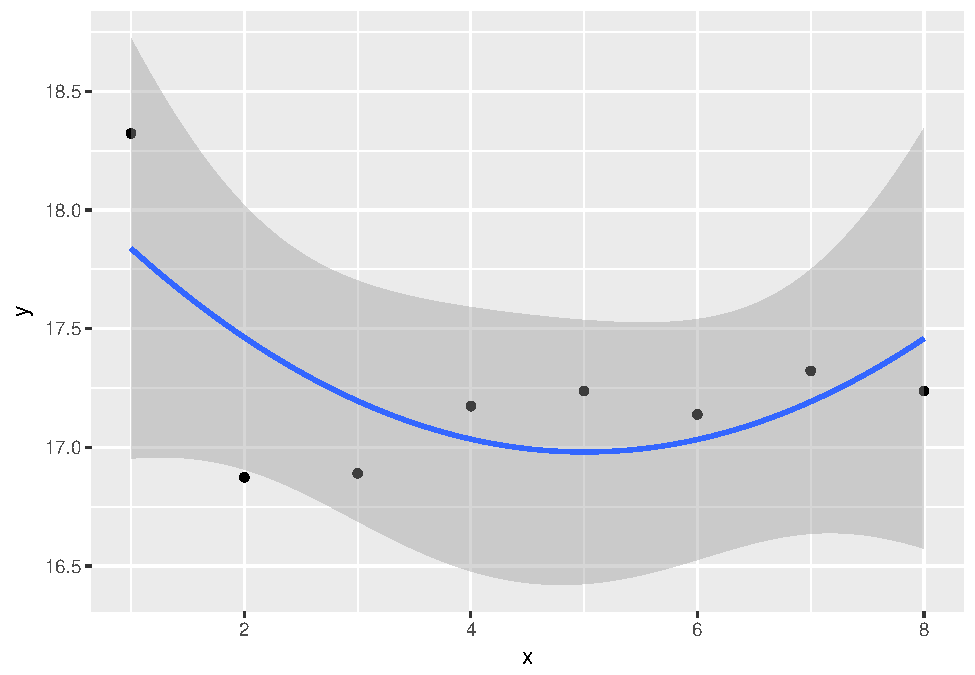
\includegraphics{CHunt_Assign12_files/figure-latex/unnamed-chunk-4-1.pdf}

Your output should show the characteristic U-shape illustrating the
tradeoff between bias and variance.


\end{document}
